\documentclass[10pt,journal,compsoc, onecolumn]{IEEEtran}

\usepackage[pdftex]{graphicx}   
\usepackage{cite}
\usepackage[utf8]{inputenc}
\usepackage[T1]{fontenc}
\usepackage{amsmath}
\usepackage{amsfonts}
\usepackage{amssymb}
\usepackage{graphicx}
\usepackage{lmodern}
\usepackage{physics}
\usepackage[left=1cm,right=1cm,top=2cm,bottom=1.5cm]{geometry}
\usepackage{siunitx}
\usepackage{fancyhdr}
\usepackage{enumerate}
\usepackage{mhchem}
\usepackage{mathrsfs}
\usepackage{mathtools}
\usepackage{graphicx}
\usepackage{float}
\usepackage{xcolor}
\usepackage{mdframed}
\usepackage{csquotes}
\usepackage{trfsigns}
\usepackage{capt-of}
\usepackage{booktabs}
\usepackage{comment}
\usepackage{amsmath}
\usepackage{algorithm}
\usepackage{amsthm}
\usepackage[noend]{algpseudocode}
\usepackage[
singlelinecheck=false % <-- important
]{caption}

\makeatletter
\def\BState{\State\hskip-\ALG@thistlm}
\makeatother

\usepackage{fixltx2e}
\usepackage{xcolor}
\def\SPSB#1#2{\rlap{\textsuperscript{\textcolor{red}{#1}}}\SB{#2}}
\def\SP#1{\textsuperscript{\textcolor{red}{#1}}}
\def\SB#1{\textsubscript{\textcolor{blue}{#1}}}

\newcommand{\subparagraph}{}
\usepackage{titlesec}

\setcounter{secnumdepth}{4}

\titleformat{\paragraph}
{\normalfont\normalsize\bfseries}{\theparagraph}{1em}{}
\titlespacing*{\paragraph}
{0pt}{3.25ex plus 1ex minus .2ex}{1.5ex plus .2ex}

\mdfdefinestyle{exercise}{
	backgroundcolor=black!10,roundcorner=8pt,hidealllines=true,nobreak
}



\newtheorem{theorem}{Theorem}[section]
\newtheorem{corollary}{corollary}[theorem]
\newtheorem{lemma}[theorem]{Lemma}
\newtheorem{definition}[theorem]{Definition}
\newtheorem{proposition}[theorem]{Proposition}
\newtheorem{remark}[theorem]{Remark}
\newtheorem{example}[theorem]{Example}






\begin{document}

\title{Spurious Quasi-Resonances for Stabilized BIE-Volume Formulations for Helmholtz Transition Problem}

\author{Frederic Jørgensen}

% TODO: Next steps:
% 1. Herleitung nochmal durchgehen und sehen dass alles richtig formulieren
% 2. Code mit Herleitung vergleichen 
% 3. Validation completen
%     a. Residuum A * sol - b plotten 
%     b. Calc scenario with general n in sol;ution e^in * phi 
%     c. Bestimmen von der p-Sache
% 4. Ergebnisse an Hiptmair



%\IEEEtitleabstractindextext{%

%\begin{abstract}

%\end{abstract}

% Note that keywords are not normally used for peerreview papers.
%\begin{IEEEkeywords}
%...\end{IEEEkeywords}}


\maketitle

\IEEEdisplaynontitleabstractindextext
\IEEEpeerreviewmaketitle

\begin{comment}
\section{Theoretical Background}

\subsubsection{Lipschitz Domain}
%Another source : https://cloudflare-ipfs.com/ipfs/bafykbzacedngw4fznskrifjbxzdjkgixzzu7mwmb4sqvsywfkq3a7mdyjclfs?filename=William%20McLean%20-%20Strongly%20Elliptic%20Systems%20and%20Boundary%20Integral%20Equations%20%20-Cambridge%20University%20Press%20%282000%29.pdf 
%Wikipedia 


\begin{remark}
Henceforth we shall require that, roughly speaking that \(\Omega\)  is locally the set of points located above the graph of some Lipschitz function and the boundary is this graph. 
\end{remark}



\begin{definition}[Lipschitz domain]
Let \(n \in \mathbb{N} .\) Let \(\Omega\) be a domain of \(\mathbb{R}^{n}\) and let \(\partial \Omega\) denote the boundary of \(\Omega .\) Then \(\Omega\) is called a Lipschitz domain if for every point \(p \in \partial \Omega\) there exists a hyperplane \(H\) of dimension \(n-1\) through \(p\), a Lipschitz-continuous function \(g: H \rightarrow \mathbb{R}\) over that hyperplane, and reals \(r>0\) and \(h>0\) such that
\begin{itemize}
    \item \(\Omega \cap C=\left\{x+y \vec{n} \mid x \in B_{r}(p) \cap H,-h<y<g(x)\right\}\)
    \item \((\partial \Omega) \cap C=\left\{x+y \vec{n} \mid x \in B_{r}(p) \cap H, g(x)=y\right\}\)
\end{itemize}
where \(\vec{n}\) is a unit vector that is normal to \(H\) and \(C:=\left\{x+y \vec{n} \mid x \in B_{r}(p) \cap H,-h<y<h\right\}\).
\end{definition}


\subsubsection{Sobolev Space}
\begin{definition}[$H^1$]
For a bounded domain \(\Omega \subset \mathbb{R}^{d}, d \in \mathbb{N}\), we define the Sobolev space \(H^{1}(\Omega):=\left\{v \in L^{2}(\Omega): \int_{\Omega}|\operatorname{grad} v(x)|^{2} \mathrm{~d} x<\infty\right\}\) as a Hilbert space with norm \(\|v\|_{H^{1}(\Omega)}^{2}:=\|v\|_{L^{2}(\Omega)}^{2}+|v|_{H^{1}(\Omega)}^{2}, \quad|v|_{H^{1}(\Omega)}^{2}:=\int_{\Omega}|\operatorname{grad} v(x)|^{2} \mathrm{~d} x\)
\end{definition}






\begin{definition}[$H^{1/2}$]

\end{definition}

\begin{definition}[$H^k_{loc}$]

\end{definition}

\subsubsection{Trace operators}
\begin{definition}[Trace operator]
A trace operator is a linear mapping from a function space on the volume domain \(\Omega\) to a function space on (parts of) the boundary \(\partial \Omega .\)
\end{definition}


\begin{definition}[(Layer) potential]
A (layer) potential is a linear mapping from a function space on \(\partial \Omega\) into a function space on the
volume domain \(\Omega .\)
\end{definition}


\begin{definition}[Dirichlet Trace]
The Dirichlet trace (operator) \(\mathrm{T}_{D}\) boils down to pointwise restriction for smooth functions:
$$
\left(\mathrm{T}_{D} w\right)(\boldsymbol{x}):=w(\boldsymbol{x}) \quad \forall \boldsymbol{x} \in \Gamma, \quad w \in C^{\infty}(\bar{\Omega}).
$$
\end{definition}
\begin{definition}[Dirichlet trace space]
The Dirichlet trace space \(H^{\frac{1}{2}}(\Gamma)\) is the Hilbert space obtained by completion of \(\left.C^{\infty}(\bar{\Omega})\right|_{\Gamma}\) with
respect to the energy norm 
$$\|\mathfrak{u}\|_{H^{\frac{1}{2}}(\Gamma)}:=\inf \left\{\|v\|_{H^{1}(\Omega)}: v \in C^{\infty}(\bar{\Omega}), \top_{D} v=\mathfrak{u}\right\},\left.\quad \mathfrak{u} \in C^{\infty}(\bar{\Omega})\right|_{\Gamma}.$$
\end{definition}

\begin{theorem}
The Dirichlet trace \(\mathrm{T}_{D}\) according can be extended to a continuous and surjective linear
operator \(\mathrm{T}_{D}: H^{1}(\Omega) \rightarrow H^{\frac{1}{2}}(\Gamma)\)
\end{theorem}

\begin{definition}[Neumann Trace]
For smooth functions the Neumann trace (operator) \(\mathrm{T}_{N}\) is defined by
$$
\left(\mathrm{T}_{N} w\right)(\boldsymbol{x}):=\operatorname{grad} w \cdot \boldsymbol{n}(\boldsymbol{x}) \quad \forall \boldsymbol{x} \in \Gamma, w \in C^{\infty}(\bar{\Omega}).
$$
\end{definition}

\begin{definition}[Neumann Trace Space]
The Neumann trace space \(H^{-\frac{1}{2}}(\Gamma)\) is the Hilbert space obtained by the completion of \(C^{0}(\Gamma)\) with respect to the norm $$\|\phi\|_{H^{-\frac{1}{2}}(\Gamma)}:=\|\widetilde{\phi}\|_{\widetilde{H}^{-1}(\Omega)}$$ where  \(\widetilde{\phi}\) is the
"extension by zero to \(\mathbb{R}^{d \text { " }}\) of \(\phi .\)
We have the definition \(\|\rho\|_{\widetilde{H}^{-1}(\Omega)}:=|u|_{H^{1}\left(\mathbb{R}^{3}\right)} \quad\) where \(u\) solves \(\quad\left\{\begin{array}{c}-\Delta u=\widetilde{\rho} \text { in } \mathbb{R}^{3} \\ u \text { satisfies decay conditions }\end{array}\right.\). 
\end{definition}

\begin{definition}[Space of function with square-integrable Laplacian]
We define the Hilbert space
$$
H(\Delta, \Omega):=\left\{v \in H^{1}(\Omega): \Delta v \in L^{2}(\Omega)\right\}
$$
with norm
$$
\|u\|_{H(\Delta, \Omega)}^{2}:=\|u\|_{H^{1}(\Omega)}^{2}+\|\Delta u\|_{L^{2}(\Omega)}^{2}, \quad u \in H(\Delta, \Omega).
$$
\end{definition}

\begin{theorem}
The Neumann trace \(\mathrm{T}_{N}\) can be extended to a continuous mapping \(\mathrm{T}_{N}: H(\Delta, \Omega) \rightarrow H^{-\frac{1}{2}}(\Gamma)\).
\end{theorem}

\begin{definition}[\(C_{\mathrm{comp}}^{\infty}\left(\mathbb{R}^{d}\right)\)]

\end{definition}


\subsubsection{Notations}
\begin{itemize}
    \item Consider a bounded Lipschitz open set $\Omega^{-} \subset \mathbb{R}^{d}$, $d=2,3$.
    \item \(\Omega^{+}:=\mathbb{R}^{d} \backslash \overline{\Omega^{-}}\)
    \item \(\Gamma:=\partial \Omega^{-}=\partial \Omega^{+}\)
    \item \(\mathbf{n}\) is the unit normal vector field on \(\Gamma\) pointing from \(\Omega^{-}\)into \(\Omega^{+}\)
    \item For any \(\varphi \in L_{\text {loc }}^{2}\left(\mathbb{R}^{d}\right)\), we let \(\varphi^{-}:=\left.\varphi\right|_{\Omega^{-}}\)and \(\varphi^{+}:=\left.\varphi\right|_{\Omega^{+}}\)
    \item \(H_{\text {loc }}^{1}\left(\Omega^{\pm}, \Delta\right):=\left\{v: \chi v \in H^{1}\left(\Omega^{\pm}\right), \Delta(\chi v) \in L^{2}\left(\Omega^{\pm}\right)\right.\)for all \(\left.\chi \in C_{\text {comp }}^{\infty}\left(\mathbb{R}^{d}\right)\right\}\)
    \item Dirichlet and Neumann trace operators\footnote{The Dirichlet trace operator boils down to pointwise restriction.}: \(\gamma_{D}^{\pm}: H_{\mathrm{loc}}^{1}\left(\Omega_{\pm}\right) \rightarrow H^{1 / 2}(\Gamma) \quad\) and \(\quad \gamma_{N}^{\pm}: H_{\mathrm{loc}}^{1}\left(\Omega_{\pm}, \Delta\right) \rightarrow H^{-1 / 2}(\Gamma)\) with \(\gamma_{D}^{\pm} v:=\left.v^{\pm}\right|_{\Gamma}\) and \(\gamma_{N}^{\pm}\)such that if \(v \in H_{\mathrm{loc}}^{2}\left(\Omega_{\pm}\right)\)then \(\gamma_{N}^{\pm} v=\mathbf{n} \cdot \gamma_{D}^{\pm}(\nabla v)\)
    \item Cauchy trace: \(\gamma_{C}^{\pm}: H_{\mathrm{loc}}^{1}\left(\Omega^{\pm}, \Delta\right) \rightarrow H^{1 / 2}(\Gamma) \times H^{-1 / 2}(\Gamma)\), \(\gamma_{C}^{\pm}:=\left(\gamma_{D}^{\pm}, \gamma_{N}^{\pm}\right)\)
    \item Sommerfeld radiation condition: \(\varphi \in C^{1}\left(\mathbb{R}^{d} \backslash B_{R}\right)\), for some ball \(B_{R}:=\{|\mathbf{x}|<R\}\), and \(\kappa>0\) satisfies this condition if \(\lim _{r \rightarrow \infty} r^{\frac{d-1}{2}}\left(\frac{\partial \varphi(\mathbf{x})}{\partial r}-\mathrm{i} \kappa \varphi(\mathbf{x})\right)=0\) in all directions. We then write \(\varphi \in \operatorname{SRC}(\kappa)\)
%\footnote{From Wikipedia: The Sommerfeld radiation condition is used to solve uniquely the Helmholtz equation. It makes sure that \"the sources must be sources, not sinks of energy. The energy which is radiated from the sources must scatter to infinity; no energy may be radiated from infinity into ... the field.\"}
\end{itemize}

\begin{theorem}[Green's first formula]
    (From Wikipedia)
    \(\int_{U}\left(\phi \nabla^{2} \psi+\nabla \phi \cdot \nabla \psi\right) \mathrm{d} U=\int_{\partial U} \phi \frac{\partial \psi}{\partial n} \mathrm{~d} S\)
\end{theorem}
\end{comment}

\section{Problem }
We start by formulating the problem. We want to investigate the occurence of spurious quasi-resonances in the variational formulation of the following Helmholtz transition problem.

\begin{definition}[Helmholtz Transmission Problem]
Find \(u \in H_{\operatorname{loc}}^{1}\left(\mathbb{R}^{d} \backslash \Gamma\right) \cap \operatorname{SRC}\left(k \sqrt{c_{o}}\right)\) 
such that

\begin{align}
    \left(\Delta+\tilde\kappa^{2} c_{i}\right) u^{-} &=0 & & \text { in } \Omega^{-}  \nonumber
    \\\left(\Delta+\tilde\kappa^{2} c_{o}\right) u^{+} &=0 & & \text { in } \Omega^{+} \label{eq:helmholtz}
    \\ \gamma_{C}^{+} u^{+} &=\gamma_{C}^{-} u^{-}+\mathbf{f} & & \text { on } \Gamma. \nonumber
\end{align}

\end{definition}

\subsection{Deriving the variational formulation}
We will now state the variational formulation of the problem in $\Omega^-$. \\
Integration by parts in $\Omega^-$ using Green's first formula implies 
$$
a(U, V) - \left(\gamma_{1}^{-} U, \gamma_{0}^{-} V\right)_{\Gamma}=0 \quad \forall v \in H^{1}\left(\Omega^{-}\right)
$$

This variational equation can be coupled to the transmission conditions using the BIE. 
As the problem is equivalent to the problem in the doctoral thesis of P. Meury (section 3) with $U_i = 0, f = 0, n(x) = c_i / c_o, 
\kappa = \tilde \kappa \sqrt{c_o}$, 
we can use the same formulation.\\
\\
The formulation is: \\ 
Find \(U \in H^{1}(\Omega), \theta \in H^{-1 / 2}(\Gamma)\) and \(p \in H^{1}(\Gamma)\) such that for all \(V \in H^{1}(\Omega), \varphi \in H^{-1 / 2}(\Gamma)\)
and \(q \in H^{1}(\Gamma)\) there holds

\begin{align}
    \mathrm{q}_{\kappa}(U, V)+\left(\mathrm{W}_{\kappa}\left(\gamma_{D}^{-} U\right), \gamma_{D}^{-} V\right)_{\Gamma}-\left((\frac{1}{2} \mathrm{ld}-\mathrm{K}_{\kappa}^{\prime})(\theta), \gamma_{D}^{-} V\right)_{\Gamma} &=g_1(V) \nonumber\\
    \left((\frac{1}{2} \mathrm{ld}-\mathrm{K}_{\kappa})\left(\gamma_{D}^{-} U\right), \varphi\right)_{\Gamma}+\left(\mathrm{V}_{\kappa}(\theta), \varphi\right)_{\Gamma}+i \overline{\eta}(p, \varphi)_{\Gamma} &=\overline{g_2(V)}(\varphi) \label{eq:variational_formulation}\\
    -\left(\mathrm{W}_{\kappa}\left(\gamma_{D}^{-} U\right), q\right)_{\Gamma}-\left((\mathrm{K}_{\kappa}^{\prime}+\frac{1}{2} \mathrm{Id})(\theta), q\right)_{\Gamma}+\mathrm{b}(p, q) &=g_3(V)(q). \nonumber
\end{align}

where we have 
$$
\begin{aligned} 
    g_1(V) &:=(f, V)_{\Omega}-\left(g_{N}, \gamma_{D}^{-} V\right)_{\Gamma}-\left(\mathrm{W}_{\kappa}\left(g_{D}\right), \gamma_{D}^{-} V\right)_{\Gamma} \\ 
    g_2(V)(\varphi) &:=\left(\varphi,\left(\mathrm{K}_{\kappa}-\frac{1}{2} \mathrm{ld}\right)\left(g_{D}\right)\right)_{\Gamma} \\ 
    g_3(V)(q) &:=\left(\mathrm{W}_{\kappa}\left(g_{D}\right), q\right)_{\Gamma}, 
\end{aligned}
$$
\(\mathrm{q}_{\kappa}(U, V):=\int_{\Omega} \operatorname{grad} U \cdot \operatorname{grad} \bar{V}-\kappa^{2} n(\mathbf{x}) U \bar{V} \mathrm{~d} \mathbf{x}\) and 
\(\mathrm{b}(p, q):=\left(\operatorname{grad}_{\Gamma} p, \operatorname{grad}_{\Gamma} q\right)_{\Gamma}+(p, q)_{\Gamma}\).

\begin{comment}
\section{How to investigate Stability}
To figure out how stable this formulation is, we use the inf-sup constant
\begin{theorem}
    Existence and uniqueness of discrete solutions \(u_{h} \in V_{h}\) and the convergence \(u_{h} \rightarrow u\) can only
hold if the sesquilinear form a satisfies a discrete inf-sup condition, cf. [89, Eq. 2.3.6]: There
exists a constant \(\gamma>0\) such that for all \(v_{h} \in V_{h}\) and the whole family \(V_{h}\) with \(h \rightarrow 0\), there
holds
$$
\sup _{0 \neq w_{h} \in V_{h}} \frac{\left|\mathrm{a}\left(v_{h}, w_{h}\right)\right|}{\left\|w_{h}\right\|_{V}} \geq \gamma\left\|v_{h}\right\|_{V}
$$ (from P.Meury thesis).
\end{theorem}
We will now investgate the reliability of the variational formulation by investigating the inf-sup constant of the sesquilinear form on the left side of the variational problem. 
\begin{definition}
$$
\gamma = \inf_{0 \neq v_h \in V_h}\sup _{0 \neq w_{h} \in V_{h}} \frac{\left|\mathrm{a}\left(v_{h}, w_{h}\right)\right|}{\left\|w_{h}\right\|_{V}\left\|v_{h}\right\|_{V}} 
$$ 
\end{definition}
\begin{remark}
    We can estimate the inf-sup constant from the minimum singular value of the Galerkin matrix (proven in P.Meury thesis).
\end{remark}

So we now derive the Galerkin Matrix to find the inf-sup constant. 
\end{comment}

\section{Derivation of Galerkin Matrix}
First, we notice that we can restrict ourselves to finding functions on $H^{\frac{1}{2}}(\Gamma)\times H^{-\frac{1}{2}}(\Gamma) \times H^1(\Gamma)$,
 since the bilinear form on the left hand side only depends on the restriction $\gamma_D^-U$.\footnote{We will see this later.} \\
Now we will further restrict this space to finite subspaces $\mathcal{H}^{\frac{1}{2}}(\Gamma), \mathcal{H}^{-\frac{1}{2}}(\Gamma)$ and $\mathcal{H}^1(\Gamma)$ 
defined by the orthonormal bases we choose for them. 
 for the finite subspaces. 
\subsection{Basis functions of $\mathcal{H}^{\frac{1}{2}}(\Gamma)$}
We make the Fourier Ansatz $V_n = V^r_n e^{i n \phi}$. 
Since $U$ must satisfy  $(\Delta + \frac{c_i}{c_o}\kappa^2) U = 0$ from eq. \ref{eq:helmholtz}, 
we have 
$$
r^2 \partial_r^2V_n^r + r \partial_r V_n^r + (r^2  \frac{c_i}{c_o}\kappa^2 - n^2)V^r_n = 0.
$$
This is Bessel's equation. Since we require convergence at the origin we have $V^r_n(r) = J_n(\sqrt{ \frac{c_i}{c_o}}\kappa r)$.


We restrict our functions to $H^{\frac{1}{2}}$ and want to get an orthonormal basis $U_n(\phi) = v_n V_n(1, \phi)$ for this space: 
$$
(U_n, U_m)_{H^{\frac{1}{2}}(\Gamma)} = \delta_{nm}
$$
This implies: 
$$
(U_n, U_m)_{H^{\frac{1}{2}}(\Gamma)} = (U_n, U_m)_{\Gamma} + (\grad_\Gamma U_n, \grad_\Gamma U_m)_{\Gamma} = \delta_{nm}
$$

$$
 = |v_n|^2 2\pi(1 + n^2) |J_n(\sqrt{ \frac{c_i}{c_o}} \kappa )|^2   \delta_{nm}  \overbrace{=}^! \delta_{nm}
$$
Therefore, we can choose real constants $v_n = \frac{1}{\sqrt{2 \pi (1 + n^2)} |J_n(\sqrt{ \frac{c_i}{c_o}} \kappa  )|}$.

\begin{comment}
\subsubsection*{Notes}
In the calculation above we used \(\nabla f = \frac{\partial f}{\partial r} \hat{\mathbf{r}}+\frac{1}{r} \frac{\partial f}{\partial \theta} \hat{\boldsymbol{\theta}}\) and eliminated the $r-$ dependency.

\textit{Note (from NumPDE Advanced):} 1. The Dirichlet trace space \(H^{\frac{1}{2}}(\Gamma)\) is the Hilbert space obtained by completion of \(\left.C^{\infty}(\bar{\Omega})\right|_{\Gamma}\) with
respect to the energy norm
$$
\|\mathfrak{u}\|_{H^{\frac{1}{2}}(\Gamma)}:=\inf \left\{\|v\|_{H^{1}(\Omega)}: v \in C^{\infty}(\bar{\Omega}), T_{D} v=\mathfrak{u}\right\},\left.\quad \mathfrak{u} \in C^{\infty}(\bar{\Omega})\right|_{\Gamma}
$$. 
\end{comment}

%2. The Dirichlet trace \(\mathrm{T}_{D}\) according to Def. 1.3.3 can be extended to a continuous and surjective linear
%$operator \(\mathrm{T}_{D}: H^{1}(\Omega) \rightarrow H^{\frac{1}{2}}(\Gamma)\)

\subsection{Basis functions for $\mathcal{H}^{-\frac{1}{2}}(\Gamma)$ and $\mathcal{H}^1(\Gamma)$}
We also pick orthonormal basis functions for $\mathcal{H}^{-\frac{1}{2}}(\Gamma)$ and $\mathcal{H}^1(\Gamma)$.
We choose $$\theta_n =w_n e^{i n \phi}\text{ where } w_n = \frac{(1 + n^2)^{\frac{1}{4}}}{\sqrt{2 \pi}}$$ for $\mathcal{H}^{\frac{1}{2}}(\Gamma)$ and for $\mathcal{H}^{-\frac{1}{2}}(\Gamma)$ we choose  $$p_n = l_n e^{i n \phi} \text{ where } l_n = \frac{1}{\sqrt{2 \pi (1+n^2)}}. $$



\subsubsection*{Notes}
See P. Meury 3.22 (Lemma )for an explanation why these bases are orthogonal 
(\textit{to be added in here later}).

\begin{comment}
Definition 3.21. For \(0 \leq s<\infty\) the space \(\mathcal{H}^{s}(\mathbb{S})\) is defined as the subspace of all functions
\(\varphi \in L^{2}(\mathbb{S})\) with the property
$$
\sum_{n \in \mathbb{Z}}\left(1+n^{2}\right)^{s}\left|\varphi_{n}\right|^{2}<\infty
$$ 
for the Fourier coefficients \(\varphi_{n}\) of \(\varphi\). With the inner product defined by
$$
(\varphi, \psi)_{\mathcal{H}^{s}(\mathbb{S})}:=\sum_{n \in \mathbb{Z}}\left(1+n^{2}\right)^{s} \varphi_{n} \overline{\psi_{n}}
$$

The Neumann trace space \(H^{-\frac{1}{2}}(\Gamma)\) is the Hilbert space obtained by the completion of \(C^{0}(\Gamma)\) with
respect to the norm
$$
\|\phi\|_{H^{-\frac{1}{2}(\Gamma)}}:=\|\widetilde{\phi}\|_{\widetilde{H}^{-1}(\Omega)}
$$

The norm is defined by this: 

Definition 1.1.80. Dual norm for source charge distributions
For \(\rho \in L^{2}(\Omega)\) let \(\widetilde{\rho} \in L^{2}\left(\mathbb{R}^{3}\right)\) be its extension by zero to \(\mathbb{R}^{3}\) and define
\(\|\rho\|_{\tilde{H}^{-1}(\Omega)}:=|u|_{H^{1}\left(\mathbb{R}^{3}\right)} \quad\) where \(u\) solves \(\left\{\begin{array}{r}-\Delta u=\widetilde{\rho} \text { in } \mathbb{R}^{3} \\ u \text { satisfies decay conditions }(1.1 .76)\end{array}\right.\)
The completion of \(L^{2}(\Omega)\) w.r.t. \(\|\cdot\|_{\tilde{H}^{-1}(\Omega)}\) yields the Hilbert space \(\widetilde{H}^{-1}(\Omega)\)

Decay condition: 
\(|u(x)|=O\left(\|x\|^{-1}\right) \quad\) and \(\quad\|\operatorname{grad} u(x)\|=O\left(\|x\|^{-2}\right) \quad\) for \(\quad\|x\| \rightarrow \infty\) (1.1.76)
\end{comment}
\section{Constructing the Galerkin Matrix}
Now let's restrict ourselves to the space $\mathcal{S}_N^{\frac{1}{2}} 
\times \mathcal{S}_N^{-\frac{1}{2}} \times \mathcal{S}_N^{1}$ where $N \in \mathbb{N}$ 
and $\mathcal{S}_N^{\frac{1}{2}}$ is the restriction to $\mathrm{span}(U_{-N}, -U_{-N+1}, ..., U_N)$ and similarly 
for $\mathcal{S}_N^{-\frac{1}{2}}$ and $\mathcal{S}_N^{1}$.
Now we can construct the Galerkin Matrix.
\subsection{Redefining the problem}
We reduce our problem to the space \(\mathcal{S}^{\frac{1}{2}} \times \mathcal{S}^{-\frac{1}{2}} \times \mathcal{S}^{1}\):
\begin{definition}[The restricted problem]
    \label{def:restricted_variational_problem}
    Find \((u, \theta, p) \in  \mathcal{S}_N^{\frac{1}{2}} \times \mathcal{S}_N^{-\frac{1}{2}} \times \mathcal{S}_N^{1}\) 
    such that for all $(V, \varphi, p) \in \mathcal{S}_N^{\frac{1}{2}} \times \mathcal{S}_N^{-\frac{1}{2}} \times \mathcal{S}_N^{1}$ there holds
    $$
    \begin{aligned}
        \mathrm{q}_{\kappa}(U, V)+\left(\mathrm{W}_{\kappa}\left(\gamma_{D}^{-} U\right), \gamma_{D}^{-} V\right)_{\Gamma}-\left((\frac{1}{2} \mathrm{ld}-\mathrm{K}_{\kappa}^{\prime})(\theta), \gamma_{D}^{-} V\right)_{\Gamma} &=g_1(V) \\
        \left((\frac{1}{2} \mathrm{ld}-\mathrm{K}_{\kappa})\left(\gamma_{D}^{-} U\right), \varphi\right)_{\Gamma}+\left(\mathrm{V}_{\kappa}(\theta), \varphi\right)_{\Gamma}+i \overline{\eta}(p, \varphi)_{\Gamma} &=\overline{g_2(V)}(\varphi) \\
        -\left(\mathrm{W}_{\kappa}\left(\gamma_{D}^{-} U\right), q\right)_{\Gamma}-\left((\mathrm{K}_{\kappa}^{\prime}+\frac{1}{2} \mathrm{Id})(\theta), q\right)_{\Gamma}+\mathrm{b}(p, q) &=g_3(V)(q).
    \end{aligned}
    $$
\end{definition}
Now let's simplify the notation of this problem a bit. First, let's extend 
$(u, \theta, p) = \sum\limits_{n = -N}^N (C^U_n U_n, C^\theta_n \theta_n, C^p_n p_n)$, 
$f_1= \sum\limits_{j = -N}^N \frac{1}{2\pi}f_1^j e^{i j \theta}$ and $f_2= \sum\limits_{j = -N}^N \frac{1}{2\pi} f_2^j e^{i j \theta}$.
\\Define $\vec{C}_n = (C^U_n, C^\theta_n, C^p_n)$.
\\Let's introduce a few new constants before deriving the Galerkin Matrix. 

\begin{definition}
    Define the notation $P^{ab}_n = (a_n, b_n)_\Gamma$ where $a_n, b_n \in L^2(\Gamma)$. 
    In particular, the following values will be helpful: 
    \begin{itemize}
        \item $P^{UU}_n = 2\pi |\tilde v_n|^2$
        \item $P^{\theta U}_n = 2\pi w_n \overline{\tilde v_n}$
        \item $P^{U\theta}_n = \overline{P^{\theta U}_n}$
        \item $P^{\theta \theta}_n = 2 \pi |w_n|^2$
        \item $P^{p \theta}_n = 2\pi l_n\overline{w_n}$
        \item $P^{Up}_n = 2\pi \tilde v_n \overline{l_n}$
        \item $P^{\theta p}_n = \overline{P^{p\theta}_n }$
    \end{itemize}
    where $\tilde v_n = J_n(\sqrt{\frac{c_i}{c_o}}\kappa )v_n$.
\end{definition}
Let's introduce the following matrix and vector: 
\begin{definition}
    \label{def:galerkin_matrix}
    $$
    A_n:= 
    \begin{pmatrix}
        (\alpha_n + \lambda_n^{(w)} P^{UU}_n)  & - (\frac{1}{2} - \lambda_n^{(K')}) P_n^{\theta U} & 0\\
        (\frac{1}{2} - \lambda_n^{(K)})P^{U\theta}_n  & \lambda^{(V)}_n P^{\theta \theta}  &  i \overline{\eta}     P^{p \theta} \\
        -\lambda_n^{(W)} P^{Up}_n  &  - (\lambda^{(K')}_n + \frac{1}{2})  P^{\theta p} & 1 
    \end{pmatrix}
    $$
    and 
    $$
    \vec{b}_n = 
    \begin{bmatrix}
       g_1(U_n)\\
        \overline{g_2}(\theta_n) \\
        g_3(p_n)
    \end{bmatrix}
    = 
    \begin{bmatrix}
        - \overline{\tilde{v_n}} f_2^n - \lambda_n^{(W)} \overline{\tilde{v_n}} f_1^n \\
        (\lambda_n^{(K)} - 0.5)  \overline{w_n} f_1^n\\
        \lambda_n^{(W)} \overline{l_n} f_1^n
    \end{bmatrix}
= f_1^n 
\underbrace{
\begin{bmatrix}
- \lambda_n^{(W)} \overline{\tilde{v_n}} \\
(\lambda_n^{(K)} - 0.5) \overline{w_n}  \\
\lambda_n^{(W)} \overline{l_n}
\end{bmatrix}}_{\vec{x_1}}
+ f_2^n
\underbrace{\begin{bmatrix}
    - \overline{\tilde{v_n}} \\
    0 \\
    0
\end{bmatrix}}_{\vec{x_1}}.
    $$
\end{definition}
The following theorem summarises the Galerkin formulation of the problem: 
\begin{theorem}
    \label{thm:galerkin_matrix}
    \((u, \theta, p) \in  \mathcal{H}^{\frac{1}{2}} \times \mathcal{H}^{-\frac{1}{2}} \times \mathcal{H}^{1}\) solves the problem in definition \ref{def:restricted_variational_problem}.
    if and only if $A_n\vec{C_n} = \vec{b}_n$ for all  $n = -N, -N + 1, ..., N$. 
\end{theorem}

Before we proof this we need the following Lemma from P. Meury doctoral thesis: 
\begin{lemma}
    The following eigenvalue equations hold for $y_n = e^{i n \phi}$:
    $$
    \begin{aligned} 
        \mathrm{V}_{\kappa}\left(y_{n}\right) &=\lambda_{n}^{(\mathrm{V})} y_{n}, & \lambda_{n}^{(\mathrm{V})} &:=\frac{i \pi}{2} J_{n}(\kappa) H_{n}^{(1)}(\kappa) \\ 
        \mathrm{K}_{\kappa}\left(y_{n}\right) &=\lambda_{n}^{(\mathrm{K})} y_{n}, & \lambda_{n}^{(\mathrm{K})} &:=\frac{i \pi \kappa}{2} J_{n}(\kappa) H_{n}^{(1)^{\prime}}(\kappa)+\frac{1}{2}=\frac{i \pi \kappa}{2} J_{n}^{\prime}(\kappa) H_{n}^{(1)}(\kappa)-\frac{1}{2} \\ 
        \mathrm{~K}_{\kappa}^{\prime}\left(y_{n}\right) &=\lambda_{n}^{\left(\mathrm{K}^{\prime}\right)} y_{n}, & \lambda_{n}^{\left(\mathrm{K}^{\prime}\right)} &:=\frac{i \pi \kappa}{2} J_{n}(\kappa) H_{n}^{(1)^{\prime}}(\kappa)+\frac{1}{2}=\frac{i \pi \kappa}{2} J_{n}^{\prime}(\kappa) H_{n}^{(1)}(\kappa)-\frac{1}{2} \\ 
        \mathcal{W}_{\kappa}\left(y_{n}\right) &=\lambda_{n}^{(\mathrm{W})} y_{n}, & \lambda_{n}^{(\mathrm{W})} &:= - \frac{i \pi \kappa^{2}}{2} J_{n}^{\prime}(\kappa) H_{n}^{(1)^{\prime}}(\kappa).
    \end{aligned}
    $$
    in particular these eigenvalue equations are satisfied for $U_n, \theta_n, p_n$.
\end{lemma}
The following formulas will also be helpful for the proof.
\begin{lemma}
    $q_\kappa(U_n, U_m) = 2 \pi  \delta_{nm}|v_n|^2\kappa  J_n(\kappa ) J_n'(\kappa ) =: \alpha_n$.
\end{lemma}


\begin{proof}[Proof of Lemma]
    We start by using Greens first formula 
    \(\int\limits_{U}(\psi \Delta \varphi+\nabla \psi \cdot \nabla \varphi) d V=\oint_{\partial U} \psi \nabla \varphi \cdot d \mathbf{S}\)
    to see that $$q_\kappa(U_n, U_m) = \int_{\Omega^-} ( \div U_n \div \overline{U_m} -  \frac{c_i}{c_o}\kappa^2U_n \overline{U_m}) $$
    $$
        = \int_{ \partial \Omega^-} \overline{U_m} \div U_n d \vec{S} - \int_{\Omega^{-}} \underbrace{( \frac{c_i}{c_o}\kappa^2 U_n + \Delta U_n)}_{=0} \overline{U_m} d \vec{S} 
    $$
    $$
        = \delta_{nm}\int_{ \partial \Omega^-} \overline{U_n} \div U_n d \vec{S}
    $$
    $$
        = \delta_{nm}|v_n|^2 \sqrt{ \frac{c_i}{c_o}} \kappa  J_n(\sqrt{ \frac{c_i}{c_o}}\kappa ) J_n'(\sqrt{ \frac{c_i}{c_o}}\kappa )  \int_{\partial \Omega^-} e^{in\phi}  e^{-in\phi} dS
    $$
    $$
        = \delta_{nm}2\pi |v_n|^2\kappa \sqrt{ \frac{c_i}{c_o}} J_n(\sqrt{ \frac{c_i}{c_o}} \kappa ) J_n'(\sqrt{ \frac{c_i}{c_o}} \kappa )
    $$
\end{proof}

\begin{remark}
    In the previous proof $U_n$ is integrated over $\Omega^-$, while $U_n$ is technically only defined on $\Gamma$. 
    However, note that, knowing the coefficients of $U_n$, it is straightforward to extend $U$ to $\Omega^-$ using our basis vectors $V_n$. 
    Also, the end result only depends on the restriction to $\Gamma$.
    \footnote{These two points is what justified the restriction of $U_n$ to $\Gamma$ in the first place.}
\end{remark}

\begin{lemma}
    $b(p_n, p_m) =  (p_n, p_m)_{H^1(\Gamma)} = \delta_{nm}$.
\end{lemma}
Now we can proof theorem \ref{thm:galerkin_matrix}
\begin{proof}
    $p_n$ is was constructed to be orthogonal w.r.t $(-, -)_{H^1(\Gamma)}$.
\end{proof}
   
\begin{proof}[Proof of theorem \ref{thm:galerkin_matrix}]
    Both sides of the problem in definition \ref{def:galerkin_matrix} are linear in $(V, \varphi, q)$. 
    Therefore the condition in the problem is satisfied for all 
    $(V, \varphi, q)\in \mathcal{S}^{\frac{1}{2}}_N  \times  \mathcal{S}^{-\frac{1}{2}}_N \times  \mathcal{S}^{1}_N$
    if and only it is satisfied for $(V, \varphi, q) \in (U_n, \theta_n, p_n) \forall n \in \{-N, -N+1, ..., N\}$.
    So we end up with $(2N + 1)$ systems of equations of the form 
    $$
    \begin{aligned}
        \mathrm{q}_{\kappa}(U, U_n)+\left(\mathrm{W}_{\kappa}\left(\gamma_{D}^{-} U\right), U_n\right)_{\Gamma}-\left((\frac{1}{2} \mathrm{ld}-\mathrm{K}_{\kappa}^{\prime})(\theta),U_n\right)_{\Gamma} &=\mathrm{f}_{2}(U_n) \\
        \left((\frac{1}{2} \mathrm{ld}-\mathrm{K}_{\kappa})\left(\gamma_{D}^{-} U\right), \theta_n\right)_{\Gamma}+\left(\mathrm{V}_{\kappa}(\theta), \theta_n\right)_{\Gamma}+i \overline{\eta}(p, \theta_n)_{\Gamma} &=\overline{g_2(V)}(\theta_n) \\
        -\left(\mathrm{W}_{\kappa}\left(\gamma_{D}^{-} U\right), p_n\right)_{\Gamma}-\left((\mathrm{K}_{\kappa}^{\prime}+\frac{1}{2} \mathrm{Id})(\theta), p_n\right)_{\Gamma}+\mathrm{b}(p, p_n) &=g_3(V)(p_n).
    \end{aligned}.
    $$
    Now, before plugging in for $(U, \theta, p)$ note the following structural feature: 
    Each of the summands of the left side of the problem has a factor that contains one of the following three bilinear forms:
    \begin{itemize}
        \item A scalar product $(a,b)_\Gamma$ of one of the entries of $(U, \theta, p)$ and a basis function. 
        \item The bilinear form $b(a,b)$ of of the entries of $(U, \theta, p)$ and a basis function. 
        \item The bilinear form $q_\kappa(a,b)$ of of the entries of $(U, \theta, p)$ and a basis function. 
    \end{itemize}
    Note that for each of these bilinear forms $s$ we have the orthogonality property $s(a_n, b_m) = 0$ for $n \neq m$, $a, b \in \{U, \theta, p\}$.
    Also considering that our basis are also eigenvectors of the BIO, this implies that for each of the $(2N + 1)$ problems all but one $x_n$ is in the kernel of the left hand side.
    Or, said more simply, the problem can be written as a blockdiagonal problem with $3 \times 3$ blocks. \\
    Plugging the relations derived in the former lemmata for $q_\kappa (U, U_n), b(p, p_n)$, 
    the BIOs and the scalar products elementary calculation yields
    $A_n x_n$ for the left hand side of the problem.  \\
    For the right, plugging in our extension for $f_1, f_2$ yields $b_n$.
    This concludes the proof. 
\end{proof} 

%Inwiefern anders von dem was P. Meury gemacht hat? 
% -> wir summieren nicht ueber die Nullstellen von Besselfunktionen 

\section{Validation}


\subsection{Solving a special case}
To validate the correctness of our derived matrix we show that it yields the correct numerical solution for a simple example. \\
Consider the special case
$$
\vec{f} = 
\begin{bmatrix}
    H_n^{(1)}(\kappa) -  J_n(\tilde c \kappa ) \\
    H_n^{\prime (1)}(\kappa) - J_n^{\prime}(\tilde c \kappa )\\
\end{bmatrix} e^{i n \phi}
$$
where $\tilde c = \sqrt{\frac{c_i}{c_o}}$ and $n =-N, -N+1, ..., N$ \\
Then the solution is 
$$
u = J_n(\tilde c \kappa r) e^{i n \phi}, x \in \Omega^-, u = H_n^{(1)}(\kappa r)e^{i n \phi}, x \in \Omega^+.
$$
This can be seen directly by plugging in.\\
\begin{remark}
Note that the discretized problem will yield the same solution as the original one 
    as the restricted space contains the analytical solution. 
\end{remark}
\begin{proposition}
    \label{prop:anasol}
    With regards to our chosen basis, the analytical solution can be written as $(U, \theta, p) = (\frac{1}{v_n} U_n, \frac{1}{w_n} \kappa H_n^{\prime(1)}(\kappa)\theta_n, 0)$. \\
    So the solution vector should be
    $$
        C_j^U = \delta_{nj}  \frac{1}{v_n}, C_j^\theta = \delta_{nj}  \frac{1}{w_n} \kappa H_n^{\prime(1)}(\kappa), C_j^p = 0, \forall j.
    $$
\end{proposition}
\begin{proof}
    \textit{still to be written out, but the main point is:} $\theta = \partial_r(u_{\Omega^+})_{|\Gamma} = - \frac{1}{w_0} \kappa_o H_1^{(1)}(\kappa_o) \theta_0 $ and $p = 0$, (from page 33 Thesis P. Meury).
\end{proof}
Let's validate whether we get the same numerical solution using our matrix $A_n$. We just use the $\vec{b}_n$ as computed above,
with $f_1^j =  \delta_{nj} 2\pi (J_n(\tilde c \kappa) - H_n^{(1)}(\kappa)), f_2^j = \delta_{nj} 2\pi (\tilde c \kappa J_1^{\prime}(\tilde c\kappa) - \kappa H_n^{\prime(1)}(\kappa))$.\\
\\
To measure how good the solution is, let's introduce the $\zeta$-number: 
\begin{definition}[ $\zeta$-number]
    For a fixed $n$ and a fixed $\kappa$, let $\vec{C}^{num}_n(\kappa)$ be the numerical solution vector to the problem \\
    $diag(A_{-N}, ..., A_N) \vec{C}^{num}_n(\kappa) = (\vec{b}_{-N}, ... , \vec{b}_{N})$. 
    Let $\vec{C}^{ana}_n(\kappa)$ be the analytical solution vector for the same problem \\
    constructed in proposition \ref{prop:anasol}.
    The $\zeta$-number is defined as 
    $$
        \zeta(\kappa)=  \max\limits_{n \in [-N, ..., N]}\frac{\|\vec{C}^{num}_n(\kappa) - \vec{C}^{ana}_n(\kappa)\|}{\|\vec{C}^{ana}_n(\kappa)\|}
    $$ 
\end{definition}
As seen in fig. \ref{fig:sol_validation}, the $\zeta$-number is negligible across all values of $\kappa$ and $n$ which validates our derivation of $A_n$ and $b_n$.
\begin{figure}
    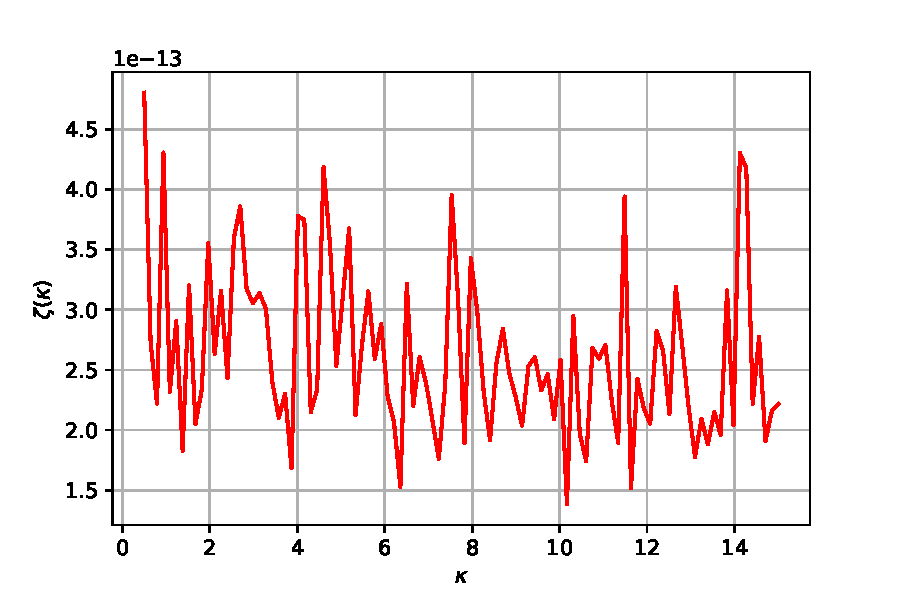
\includegraphics[width=0.5\textwidth]{scenario1SolVal.pdf}
    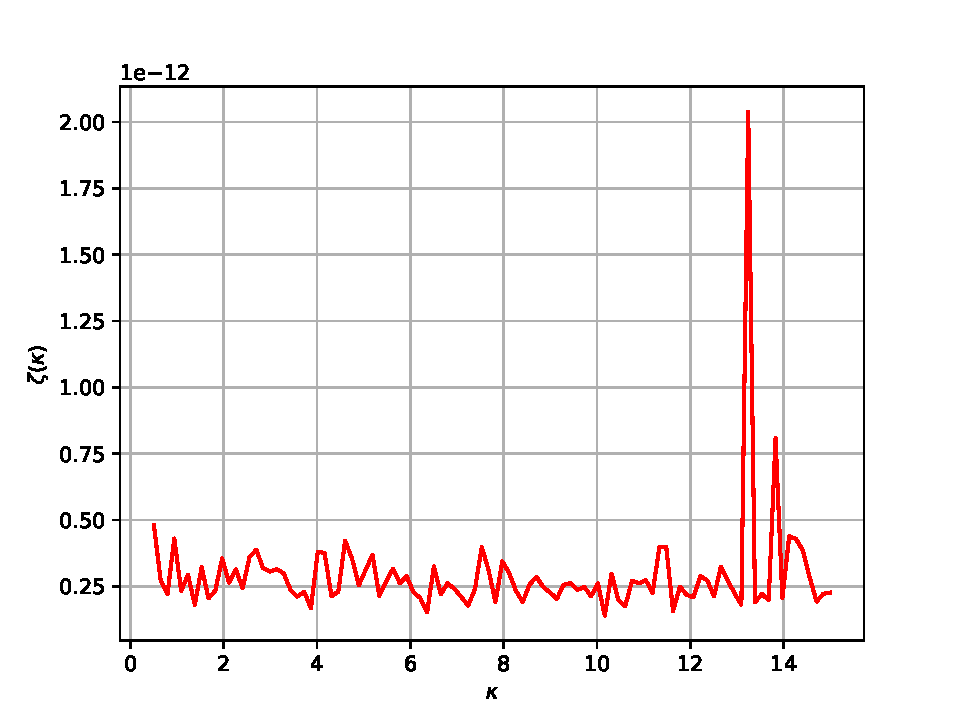
\includegraphics[width=0.5\textwidth]{scenario2SolVal.pdf}
    \caption{Maximum relative residuum of the numerical solution by wave number. 
    On the left plot we have $c_i = 1, c_o = 3$ 
    and on the right plot we have $c_i = 3, c_o = 1.$
    We always use $N = 100$ from here on.}
    \label{fig:sol_validation}
\end{figure}
\subsection{p = 0}
We validate our matrix $A$ with another method, using the following remark from the doctoral
thesis from P.Meury:
\begin{remark}
    \label{rem:pzero}
At second glance, we realise that \(p=0\), if \((U, \theta)\) solve the problem. \\
\end{remark}
Let's assume $A_n$ is invertible\footnote{This is fair to assume for most frequencies since the variational problem is supposed to have a unique solution.}.
We can use the remark to validate that our derived matrix $A_n$ is correct, using the following proposition:
\begin{proposition}
    Let $V_{\vec{b}} := span( \vec{x}_1, \vec{x}_2)$ and let
     $P_{V_{\vec{b}}}$ be the projector onto $V_{\vec{b}}$.
     Let $P_3$ be the projector onto $(0, 0, 1)$.
     Then $P_3A_n^{-1}P_{V_{\vec{b}}} = 0$.
\end{proposition}
\begin{proof}
    Because of the remark \ref{rem:pzero}, every solution of  $A_n \vec{x} = \vec{b}_n$ satisfies $x_3 = 0$
    where $\vec{b} \in V_{\vec{b}}$. \\
    Therefore $ V_{\vec{b}} \subset Ker(P_3A_n^{-1})$. 
    Since $\vec{x}_1, \vec{x}_2$ are linearly independent, $\mathrm{dim} V_{\vec{b}} =2$, which implies $ V_{\vec{b}} = Ker(P_3A_n^{-1})$.
    So $P_3A_n^{-1}P_{V_{\vec{b}}} = 0$.
\end{proof}
    

Let's check whether this is actually satisfied 
by calculating the euclidian matrix norm of $A$ for a range of $\kappa$ values. 

As we see in fig \ref{fig:p_validation}, this is satisfied which is another validation of our matrix $A$.

\begin{figure}
    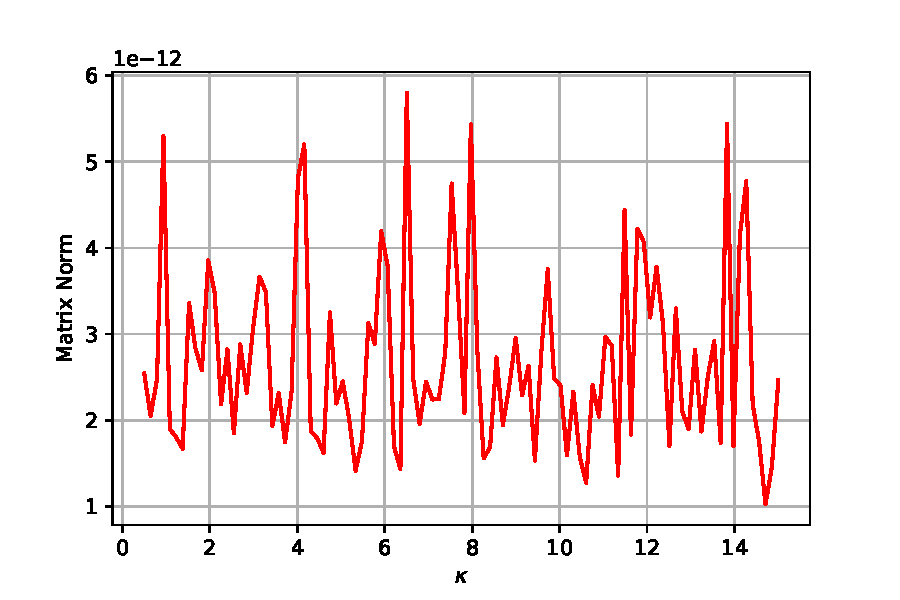
\includegraphics[width=0.5\textwidth]{scenario1PVal.pdf}
    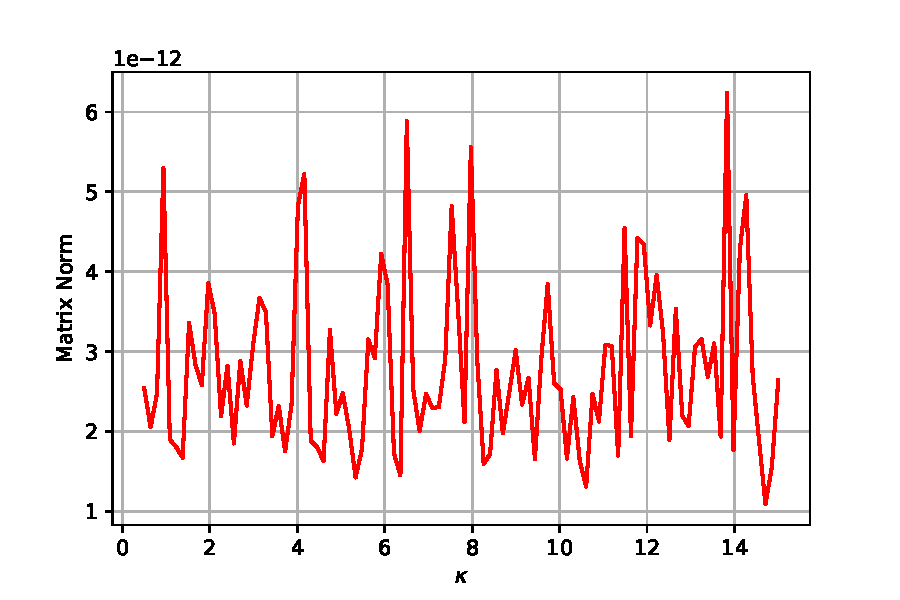
\includegraphics[width=0.5\textwidth]{scenario2PVal.pdf}
    \caption{Euclidian matrix norm of composed matrix  $P_3A_n^{-1}P_{V_{\vec{b}}}$. 
    On the left plot we have $c_i = 1, c_o = 3$ 
    and on the right plot we have $c_i = 3, c_o = 1.$}
   \label{fig:p_validation}
\end{figure}


\section{Numerical Results}
Now let's investigate maximal singular value of $A = diag(A_{-N}, A_{-N + 1}, ..., A_{N})$. 
Again, we look at the scenarios where $c_i = 1, c_o = 3$ and vice versa (fig. \ref{fig:max_sing_val})
We see that the peaks often coincide with the zeros of the Bessel function. 

\begin{figure}
    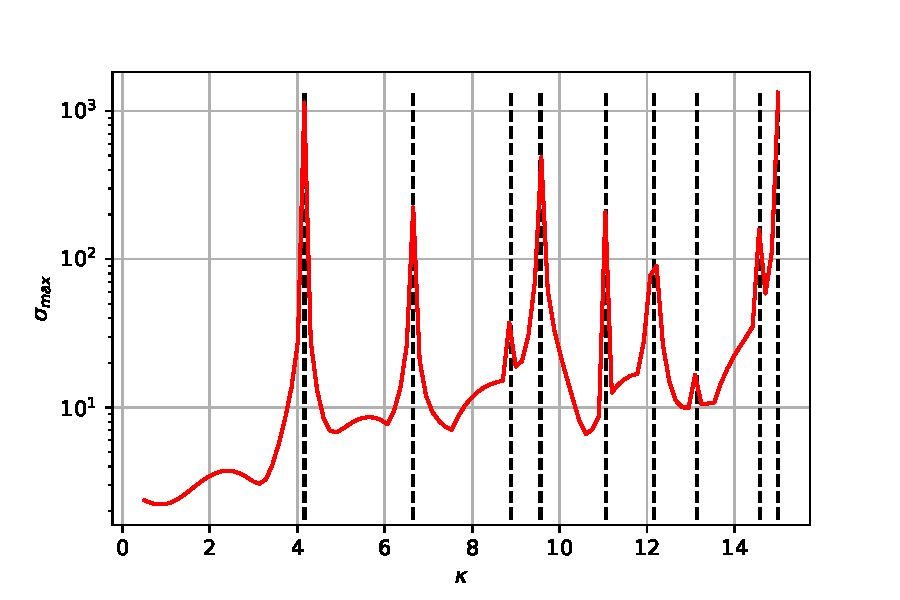
\includegraphics[width=0.5\textwidth]{scenario1MaximumSingVal.pdf}
    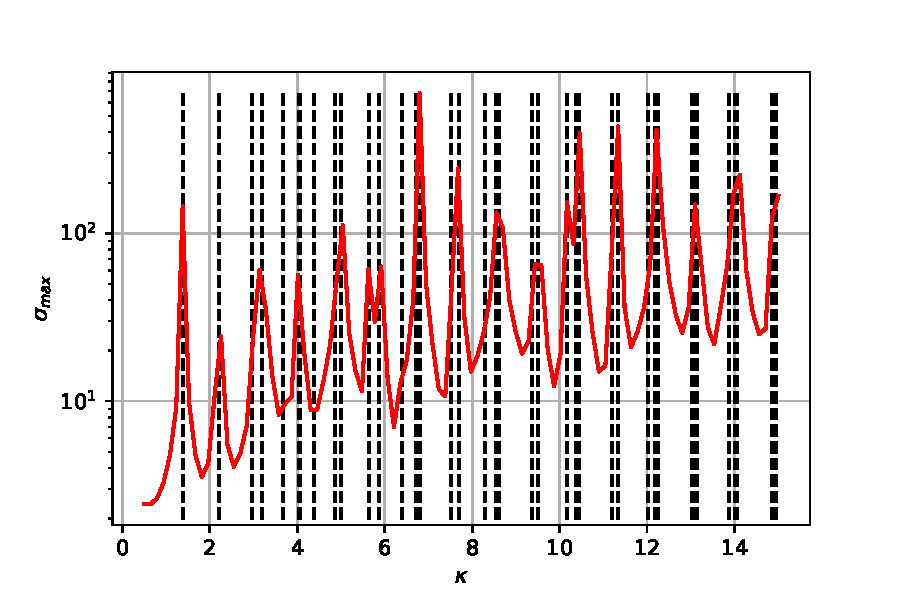
\includegraphics[width=0.5\textwidth]{scenario2MaximumSingVal.pdf}
    \caption{Maximum singular value of the matrix $diag(A_n)$ by wave number $\kappa$. 
    On the left plot we have $c_i = 1, c_o = 3$ 
    and on the right plot we have $c_i = 3, c_o = 1.$} The vertical dashed lines correspond to zeros of the BEssel functions. 
   \label{fig:max_sing_val}
\end{figure}
We can also consider the minimum singular value (fig. \ref{fig:min_sing_val}).
\begin{figure}
    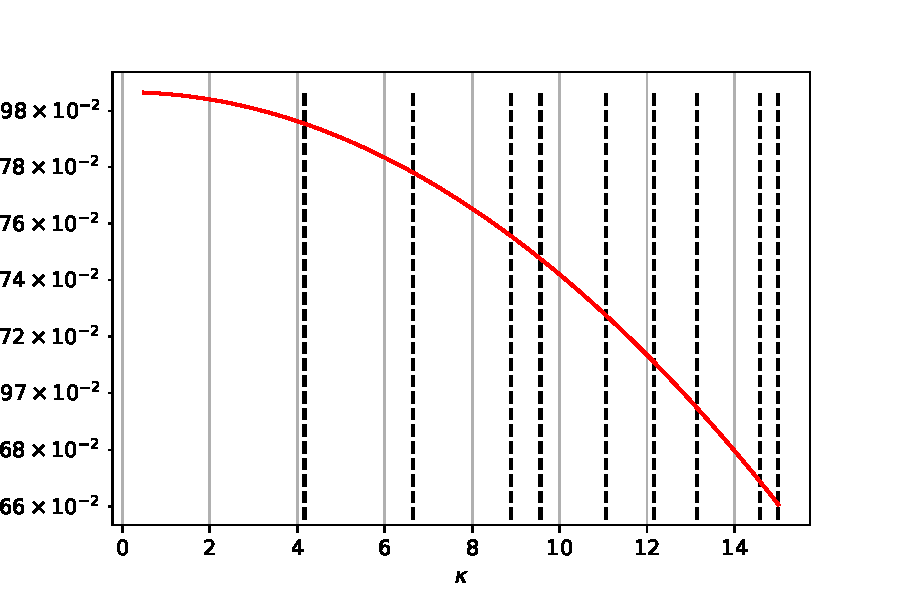
\includegraphics[width=0.5\textwidth]{scenario1MinimumSingVal.pdf}
    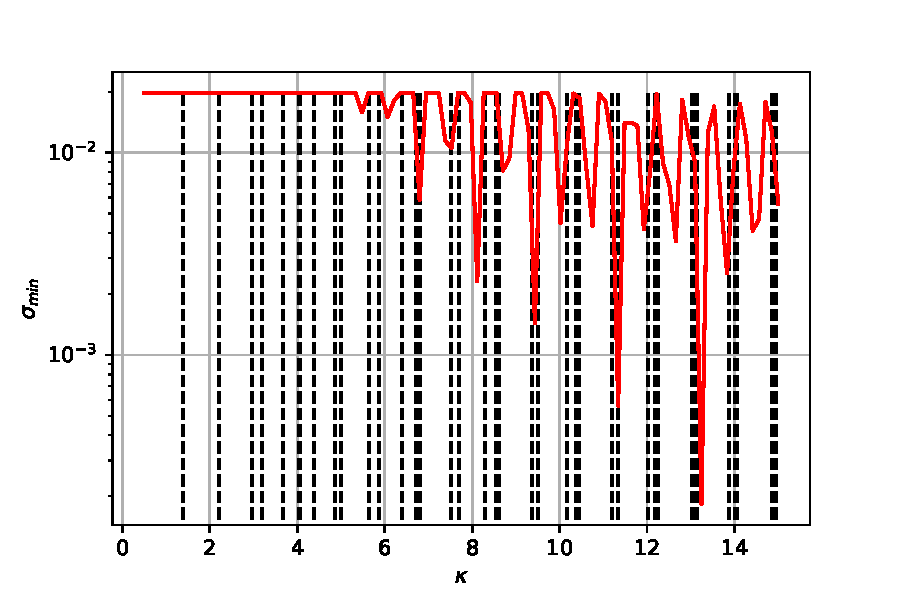
\includegraphics[width=0.5\textwidth]{scenario2MinimumSingVal.pdf}
    \caption{Maximum singular value of the matrix $diag(A_n)$ by wave number $\kappa$. 
    On the left plot we have $c_i = 1, c_o = 3$ 
    and on the right plot we have $c_i = 3, c_o = 1.$ Again, the vertical dashed lines correspond to zeros of the BEssel functions. }
   \label{fig:min_sing_val}
\end{figure}
Finally, let's consider the ratio of the minimum and maximum singular value (fig. \ref{fig:ratio_sing_val}).
\begin{figure}
    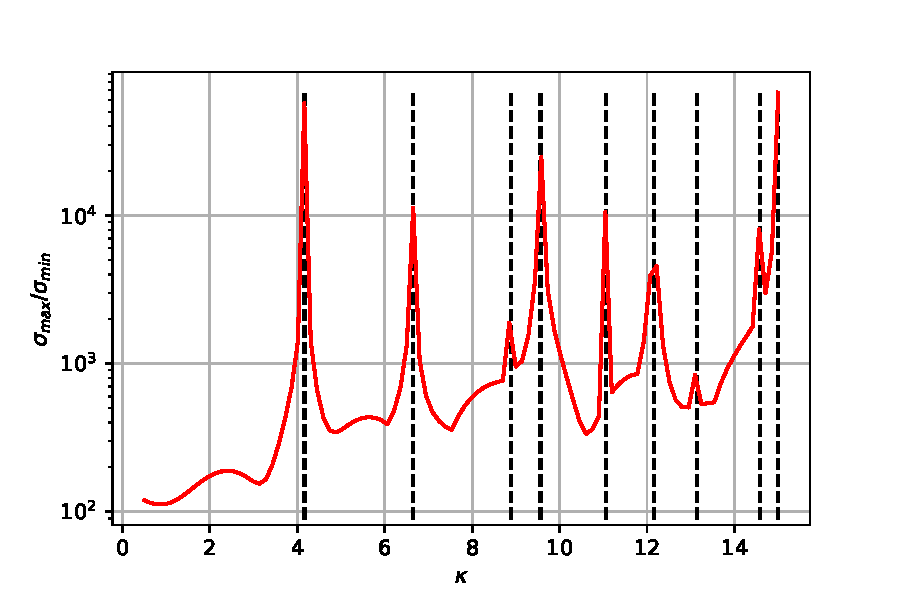
\includegraphics[width=0.5\textwidth]{scenario1Ratio.pdf}
    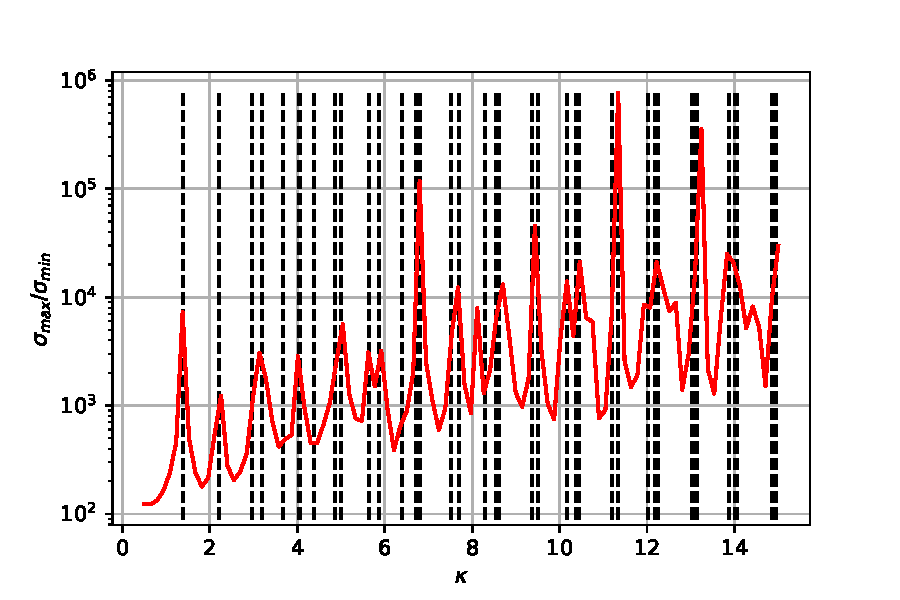
\includegraphics[width=0.5\textwidth]{scenario2Ratio.pdf}
    \caption{Ratio of Maximum and Minimum singular value of the matrix $diag(A_n)$ by wave number $\kappa$. 
    On the left plot we have $c_i = 1, c_o = 3$ 
    and on the right plot we have $c_i = 3, c_o = 1.$ The vertical dashed lines correspond to zeros of the BEssel functions. }
   \label{fig:ratio_sing_val}
\end{figure}
We see that in the case $c_i = 1, c_o =3$, where the solution operator has weaker resonances resonances, 
the resonances from our matrix operator or also less strong 
than in the case $c_i = 3, c_o =1$.


%
%\bibliography{bib}
%\bibliographystyle{ieeetr}


\end{document}

OLD STuff 

\subsection{Even more special case}
In addition to the assumptions above, pick $c_o = 1$, $\eta = 1$, and $\kappa = 5.502$ (then $J_0(\kappa) = 0$).\\
Then we have $\lambda_0^{(V)} =0$, $\lambda_n^{(K)} = \lambda_n^{(K')} = 1/2$. For easier notation write $\lambda_n^{(W)} =: \nu$.
Now we have
$$
A_0 = 
\begin{pmatrix}
    \alpha_0 + \nu P^{UU}_0  & 0 & 0\\
    0 & 0  &  i P^{p \theta} \\
    -\nu P^{Up}_0  &  -P_0^{\theta p} & 1 
\end{pmatrix}.
$$
Moreover we have 
$$
b_0 = 2 \pi H_0^{(1)}(\kappa)
\begin{bmatrix}
    -\nu \overline{\tilde{v_0}} \\
    0  \\
    \nu \overline{l_0}
\end{bmatrix}
+  2 \pi (H_1^{(1)}(\kappa) - J_1^{(1)}(\kappa))
\begin{bmatrix}
    - \overline{\tilde{v_0}} \\
    0 \\
    0
\end{bmatrix}.
$$

We have 
$$
A_0^{-1} = 
\begin{pmatrix}
    (\alpha_n + \nu P^{UU}_n)^{-1} & 0 & 0 \\
    - \frac{\nu P_0^{(Up)}}{( \alpha_0 + \nu P^{UU}_0) P_0^{\theta p}} & -\frac{i}{(P_0^{\theta p})^2} & -\frac{1}{P_0^{\theta p}} \\
    0 & - \frac{i}{P^{p \theta}_0} & 0 
\end{pmatrix}.
$$
So $
x = A_0^{-1} b_0 =  ...
\begin{pmatrix}
    %TODO: VON HIER WEITER UND HERAUSFINDEN WARUM NICHT ANALYTISCHE LOESUNG RAUSKOMMT. Eventuell divergiert v_0? 
    % Andere v_n  benutzen die nicht divergieren in der Naehe von Resonanzne? Also zB auf ganzem Kreis normieren? Dann faellt eventuell auch ein J_n oben weg 


\end{pmatrix}
$

\section{Defining the problem}
\subsection{Basic Definitions}
\subsubsection{Lipschitz Domain}
%Another source : https://cloudflare-ipfs.com/ipfs/bafykbzacedngw4fznskrifjbxzdjkgixzzu7mwmb4sqvsywfkq3a7mdyjclfs?filename=William%20McLean%20-%20Strongly%20Elliptic%20Systems%20and%20Boundary%20Integral%20Equations%20%20-Cambridge%20University%20Press%20%282000%29.pdf 
%Wikipedia 


\begin{remark}
Henceforth we shall require that, roughly speaking that \(\Omega\)  is locally the set of points located above the graph of some Lipschitz function and the boundary is this graph. 
\end{remark}



\begin{definition}[Lipschitz domain]
Let \(n \in \mathbb{N} .\) Let \(\Omega\) be a domain of \(\mathbb{R}^{n}\) and let \(\partial \Omega\) denote the boundary of \(\Omega .\) Then \(\Omega\) is called a Lipschitz domain if for every point \(p \in \partial \Omega\) there exists a hyperplane \(H\) of dimension \(n-1\) through \(p\), a Lipschitz-continuous function \(g: H \rightarrow \mathbb{R}\) over that hyperplane, and reals \(r>0\) and \(h>0\) such that
\begin{itemize}
    \item \(\Omega \cap C=\left\{x+y \vec{n} \mid x \in B_{r}(p) \cap H,-h<y<g(x)\right\}\)
    \item \((\partial \Omega) \cap C=\left\{x+y \vec{n} \mid x \in B_{r}(p) \cap H, g(x)=y\right\}\)
\end{itemize}
where \(\vec{n}\) is a unit vector that is normal to \(H\) and \(C:=\left\{x+y \vec{n} \mid x \in B_{r}(p) \cap H,-h<y<h\right\}\).
\end{definition}


\subsubsection{Sobolev Space}
\begin{definition}[$H^1$]
For a bounded domain \(\Omega \subset \mathbb{R}^{d}, d \in \mathbb{N}\), we define the Sobolev space \(H^{1}(\Omega):=\left\{v \in L^{2}(\Omega): \int_{\Omega}|\operatorname{grad} v(x)|^{2} \mathrm{~d} x<\infty\right\}\) as a Hilbert space with norm \(\|v\|_{H^{1}(\Omega)}^{2}:=\|v\|_{L^{2}(\Omega)}^{2}+|v|_{H^{1}(\Omega)}^{2}, \quad|v|_{H^{1}(\Omega)}^{2}:=\int_{\Omega}|\operatorname{grad} v(x)|^{2} \mathrm{~d} x\)
\end{definition}






\begin{definition}[$H^{1/2}$]

\end{definition}

\begin{definition}[$H^k_{loc}$]

\end{definition}

\subsubsection{Trace operators}
\begin{definition}[Trace operator]
A trace operator is a linear mapping from a function space on the volume domain \(\Omega\) to a function space on (parts of) the boundary \(\partial \Omega .\)
\end{definition}


\begin{definition}[(Layer) potential]
A (layer) potential is a linear mapping from a function space on \(\partial \Omega\) into a function space on the
volume domain \(\Omega .\)
\end{definition}


\begin{definition}[Dirichlet Trace]
The Dirichlet trace (operator) \(\mathrm{T}_{D}\) boils down to pointwise restriction for smooth functions:
$$
\left(\mathrm{T}_{D} w\right)(\boldsymbol{x}):=w(\boldsymbol{x}) \quad \forall \boldsymbol{x} \in \Gamma, \quad w \in C^{\infty}(\bar{\Omega}).
$$
\end{definition}
\begin{definition}[Dirichlet trace space]
The Dirichlet trace space \(H^{\frac{1}{2}}(\Gamma)\) is the Hilbert space obtained by completion of \(\left.C^{\infty}(\bar{\Omega})\right|_{\Gamma}\) with
respect to the energy norm 
$$\|\mathfrak{u}\|_{H^{\frac{1}{2}}(\Gamma)}:=\inf \left\{\|v\|_{H^{1}(\Omega)}: v \in C^{\infty}(\bar{\Omega}), \top_{D} v=\mathfrak{u}\right\},\left.\quad \mathfrak{u} \in C^{\infty}(\bar{\Omega})\right|_{\Gamma}.$$
\end{definition}

\begin{theorem}
The Dirichlet trace \(\mathrm{T}_{D}\) according can be extended to a continuous and surjective linear
operator \(\mathrm{T}_{D}: H^{1}(\Omega) \rightarrow H^{\frac{1}{2}}(\Gamma)\)
\end{theorem}

\begin{definition}[Neumann Trace]
For smooth functions the Neumann trace (operator) \(\mathrm{T}_{N}\) is defined by
$$
\left(\mathrm{T}_{N} w\right)(\boldsymbol{x}):=\operatorname{grad} w \cdot \boldsymbol{n}(\boldsymbol{x}) \quad \forall \boldsymbol{x} \in \Gamma, w \in C^{\infty}(\bar{\Omega}).
$$
\end{definition}

\begin{definition}[Neumann Trace Space]
The Neumann trace space \(H^{-\frac{1}{2}}(\Gamma)\) is the Hilbert space obtained by the completion of \(C^{0}(\Gamma)\) with respect to the norm $$\|\phi\|_{H^{-\frac{1}{2}}(\Gamma)}:=\|\widetilde{\phi}\|_{\widetilde{H}^{-1}(\Omega)}$$ where  \(\widetilde{\phi}\) is the
"extension by zero to \(\mathbb{R}^{d \text { " }}\) of \(\phi .\)
We have the definition \(\|\rho\|_{\widetilde{H}^{-1}(\Omega)}:=|u|_{H^{1}\left(\mathbb{R}^{3}\right)} \quad\) where \(u\) solves \(\quad\left\{\begin{array}{c}-\Delta u=\widetilde{\rho} \text { in } \mathbb{R}^{3} \\ u \text { satisfies decay conditions }\end{array}\right.\). 
\end{definition}

\begin{definition}[Space of function with square-integrable Laplacian]
We define the Hilbert space
$$
H(\Delta, \Omega):=\left\{v \in H^{1}(\Omega): \Delta v \in L^{2}(\Omega)\right\}
$$
with norm
$$
\|u\|_{H(\Delta, \Omega)}^{2}:=\|u\|_{H^{1}(\Omega)}^{2}+\|\Delta u\|_{L^{2}(\Omega)}^{2}, \quad u \in H(\Delta, \Omega).
$$
\end{definition}

\begin{theorem}
The Neumann trace \(\mathrm{T}_{N}\) can be extended to a continuous mapping \(\mathrm{T}_{N}: H(\Delta, \Omega) \rightarrow H^{-\frac{1}{2}}(\Gamma)\).
\end{theorem}

\begin{definition}[\(C_{\mathrm{comp}}^{\infty}\left(\mathbb{R}^{d}\right)\)]

\end{definition}


\subsubsection{Notations}
\begin{itemize}
    \item Consider a bounded Lipschitz open set $\Omega^{-} \subset \mathbb{R}^{d}$, $d=2,3$.
    \item \(\Omega^{+}:=\mathbb{R}^{d} \backslash \overline{\Omega^{-}}\)
    \item \(\Gamma:=\partial \Omega^{-}=\partial \Omega^{+}\)
    \item \(\mathbf{n}\) is the unit normal vector field on \(\Gamma\) pointing from \(\Omega^{-}\)into \(\Omega^{+}\)
    \item For any \(\varphi \in L_{\text {loc }}^{2}\left(\mathbb{R}^{d}\right)\), we let \(\varphi^{-}:=\left.\varphi\right|_{\Omega^{-}}\)and \(\varphi^{+}:=\left.\varphi\right|_{\Omega^{+}}\)
    \item \(H_{\text {loc }}^{1}\left(\Omega^{\pm}, \Delta\right):=\left\{v: \chi v \in H^{1}\left(\Omega^{\pm}\right), \Delta(\chi v) \in L^{2}\left(\Omega^{\pm}\right)\right.\)for all \(\left.\chi \in C_{\text {comp }}^{\infty}\left(\mathbb{R}^{d}\right)\right\}\)
    \item Dirichlet and Neumann trace operators\footnote{The Dirichlet trace operator boils down to pointwise restriction.}: \(\gamma_{D}^{\pm}: H_{\mathrm{loc}}^{1}\left(\Omega_{\pm}\right) \rightarrow H^{1 / 2}(\Gamma) \quad\) and \(\quad \gamma_{N}^{\pm}: H_{\mathrm{loc}}^{1}\left(\Omega_{\pm}, \Delta\right) \rightarrow H^{-1 / 2}(\Gamma)\) with \(\gamma_{D}^{\pm} v:=\left.v^{\pm}\right|_{\Gamma}\) and \(\gamma_{N}^{\pm}\)such that if \(v \in H_{\mathrm{loc}}^{2}\left(\Omega_{\pm}\right)\)then \(\gamma_{N}^{\pm} v=\mathbf{n} \cdot \gamma_{D}^{\pm}(\nabla v)\)
    \item Cauchy trace: \(\gamma_{C}^{\pm}: H_{\mathrm{loc}}^{1}\left(\Omega^{\pm}, \Delta\right) \rightarrow H^{1 / 2}(\Gamma) \times H^{-1 / 2}(\Gamma)\), \(\gamma_{C}^{\pm}:=\left(\gamma_{D}^{\pm}, \gamma_{N}^{\pm}\right)\)
    \item Sommerfeld radiation condition: \(\varphi \in C^{1}\left(\mathbb{R}^{d} \backslash B_{R}\right)\), for some ball \(B_{R}:=\{|\mathbf{x}|<R\}\), and \(\kappa>0\) satisfies this condition if \(\lim _{r \rightarrow \infty} r^{\frac{d-1}{2}}\left(\frac{\partial \varphi(\mathbf{x})}{\partial r}-\mathrm{i} \kappa \varphi(\mathbf{x})\right)=0\) in all directions. We then write \(\varphi \in \operatorname{SRC}(\kappa)\)
\footnote{From Wikipedia: The Sommerfeld radiation condition is used to solve uniquely the Helmholtz equation. It makes sure that \"the sources must be sources, not sinks of energy. The energy which is radiated from the sources must scatter to infinity; no energy may be radiated from infinity into ... the field.\"}
\end{itemize}
\subsection{Definition of the problem}

\begin{definition}
Given \(c_i, c_o>0\) and frequency \(k>0\), the Helmholtz transmission scattering problem is
that of finding the complex amplitude \(u\) of the sound pressure, with \(u \in H_{\text {loc }}^{1}\left(\mathbb{R}^{d} \backslash \Gamma\right)\) the solution
of \(\begin{aligned}\left(\Delta+k^{2} c_i\right) u^{-} &=0 & & \text { in } \Omega^{-} \\\left(\Delta+k^{2} c_o\right) u^{+} &=0 & & \text { in } \Omega^{+} \\ \gamma_{C}^{-} u^{-} &=\gamma_{C}^{+} u^{+}+\gamma_{C}^{\pm} u^{I} & & \text { on } \Gamma \\ u^{+} & \in \operatorname{SRC}\left(k \sqrt{c_o}\right), & & \end{aligned}\)
where the incident wave\footnote{Solution if transmission material would not be there.} \(u^{I}\) is an entire solution of the homogeneous Helmholtz equation in \(\mathbb{R}^{d}\) 
$$\left(\Delta+k^{2} c_o\right) u^{I}=0 \quad \text{ in } \mathbb{R}^{d}\
$$

\end{definition}


In principle, the jump \(\gamma_{C}^{+} u^{+}-\gamma_{C}^{-} u^{-}\)of the Cauchy trace of \(u\) across \(\Gamma\) can be more general than the Cauchy trace of an incident wave. This leads to the following generic Helmholtz transmission problem.


\begin{definition}
Given positive real numbers \(k, c_i\), and \(c_o\) and \(\mathbf{f} \in H^{1 / 2}(\Gamma) \times H^{-1 / 2}(\Gamma)\), find \(u \in H_{\mathrm{loc}}^{1}\left(\mathbb{R}^{d} \backslash \Gamma\right) \cap \operatorname{SRC}\left(k \sqrt{c_o}\right)\) such that,
\(\begin{aligned}\left(\Delta+k^{2} c_i\right) u^{-} &=0 & & i n \Omega^{-} \\\left(\Delta+k^{2} c_o\right) u^{+} &=0 & & i n \Omega^{+} \\ \gamma_{C}^{-} u^{-} &=\gamma_{C}^{+} u^{+}+\mathbf{f} & & \text { on } \Gamma \end{aligned}\)
\end{definition}
\begin{lemma}
The solution of the transmission problem of Definition \(1.1\) exists and is unique.
Moreover, if \(\mathbf{f} \in H^{1}(\Gamma) \times L^{2}(\Gamma)\) then \(\gamma_{C}^{\pm} u^{\pm} \in H^{1}(\Gamma) \times L^{2}(\Gamma)\)
\end{lemma}

\section{Solution operators}
\begin{definition}
Given positive real numbers \(k, c_{i}\), and \(c_{o}\), let
$$
S\left(c_{i}, c_{o}\right) \mathbf{f}:=\gamma_{C}^{-} u
$$
where \(u \in H_{\mathrm{loc}}^{1}\left(\mathbb{R}^{d} \backslash \Gamma\right) \cap \operatorname{SRC}\left(k \sqrt{c_{o}}\right)\) is the solution of the Helmholtz transmission problem with $c_i = c_i$. According to the earlier lemmas this is well-defined.
\end{definition}



%\begin{definition}
%We introduce the abbreviations \(S_{i o}:=S\left(c_i, c_o\right) \quad\) and \(\quad S_{o i}:=S\left(c_o, c_i\right)\). 
%\end{definition}
